\documentclass[a4paper,12pt]{article}
\usepackage{multirow}
\usepackage{graphicx} % Required for inserting images
\usepackage{amsmath,amssymb,amsfonts}
\usepackage{subcaption}
% Use Times New Roman font
\usepackage{times}
\usepackage[a4paper, top=1in, bottom=0.8in, left=1.1in, right=0.8in]{geometry}
\usepackage{float}
\usepackage{listings}
\usepackage{xcolor} % For customizing code colors
\setlength{\parindent}{0pt}
\usepackage{titlesec} % Add this to your preamble
\titleformat{\section}
{\normalfont\large\bfseries}{\thesection}{1em}{}
% Set spacing for sections
\titlespacing*{\section}
{0pt}  % Left spacing
{1ex} % Space before (adjust this value)
{1ex}  % Space after (adjust this value)
\begin{document}
	\section{Experiment No. 7}
	
	
	\section{Experiment Title }
	Design and Analyze 2×2 and 3×3 Crossbar Switch and Barrel Shifter on MICROWIND 3.0
	\section{Objective}
	The main objectives of this report are:
	\begin{itemize}
		\item To design and simulate 2×2 and 3×3 crossbar switch and barrel shifter on Microwind 3.0
		\item To observe and analyze the behaviour of the outputs of the designed circuits.
	
	\end{itemize}
	
	\section{Theory}
	\subsection{2X2 Crossbar Switch}
	A crossbar switch is a network of individual switches connecting a set of inputs to a set of outputs, arranged in a matrix layout. For example, if a crossbar switch has M inputs and N outputs, it forms an M × N matrix with connection points, called crosspoints, where connections can be made. Each crosspoint has a switch, which, when closed, connects a specific input to a specific output. This setup makes the crossbar a single-layer, non-blocking switch, meaning multiple connections can be made without interference.A 2X2 Crossbar Switch has two inputs and two outputs, allowing each input to connect to any output. It has four "crosspoints" or connection points, which can be turned on to link specific inputs to specific outputs.
		\subsection{3X3 Crossbar Switch}
		A 3x3 crossbar switch extends the matrix to three inputs and three
		outputs, introducing nine switching points.
			\begin{figure}[H]
			\centering
			\begin{subfigure}[t]{0.49\textwidth}
				\centering
			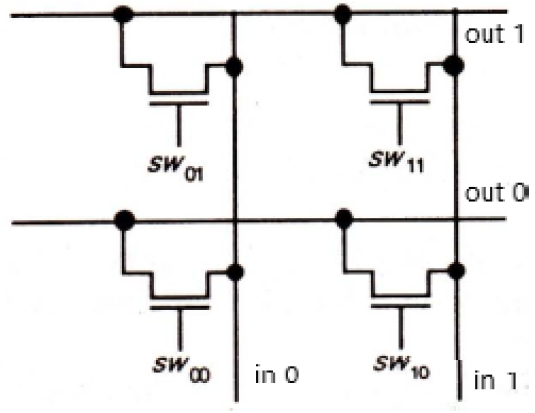
\includegraphics[width=1\linewidth]{Images/1}
				\caption{2X2 Crossbar Switch}
			\end{subfigure}
			\hfill
			\begin{subfigure}[t]{0.48\textwidth}
				\centering
			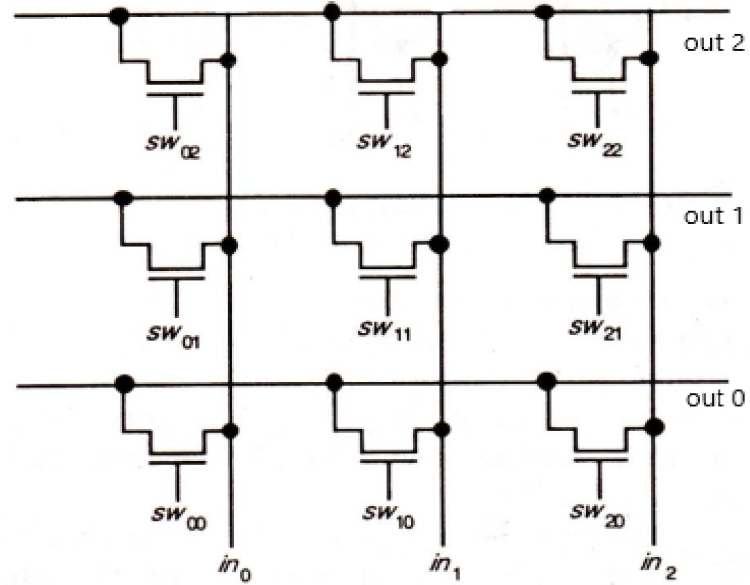
\includegraphics[width=1\linewidth]{Images/2}
				\caption{ 3X3 Crossbar Switch}
			\end{subfigure}
		\end{figure}
	\newpage
		\subsection{2X2 Barrel Shifter}
	A barrel shifter is a circuit that moves data left or right by a certain number of positions all at once. In a 2x2 barrel shifter, you can shift the data one or two positions in a single clock cycle. This circuit uses a set of multiplexers that are controlled by select lines. There are two shifter lines, called shift 0 and shift 1, which work together to shift the bits as needed. This setup allows the barrel shifter to quickly and efficiently change the position of the data.
		\begin{figure}[H]
		\centering
		\begin{subfigure}[t]{0.49\textwidth}
			\centering
			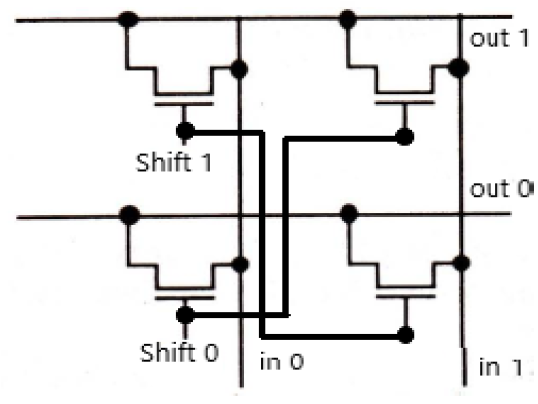
\includegraphics[width=1\linewidth]{Images/3}
			\caption{2X2 Barrel Shifter}
		\end{subfigure}
		\hfill
		\begin{subfigure}[t]{0.48\textwidth}
			\centering
			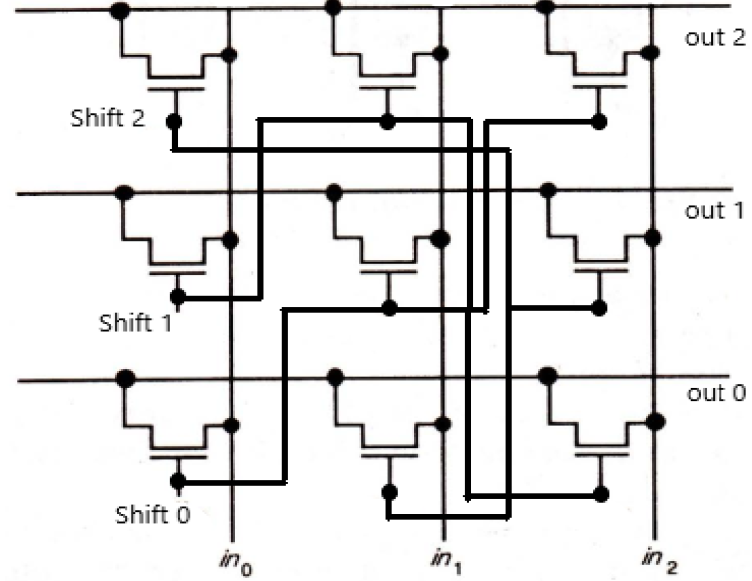
\includegraphics[width=1\linewidth]{Images/4}
			\caption{ 3X3 Barrel Shifter}
		\end{subfigure}
	\end{figure}
		\subsection{3X3 Barrel Shifter}
		Like the 2x2 barrel shifter, a 3x3 barrel shifter also shifts data but can move it up to three positions. It has three shifting lines: shift 0, shift 1, and shift 2. These lines are interconnected, allowing the shifter to move bits—bit 0, bit 1, and bit 2—according to the selected shift operation. This setup enables the 3x3 barrel shifter to efficiently shift data to the left or right by one, two, or three positions in a single operation.
	\newpage
	\section{Schematic Layout }
	\subsection{2X2 Barrel Shifter}
	\begin{figure}[H]
		\centering
		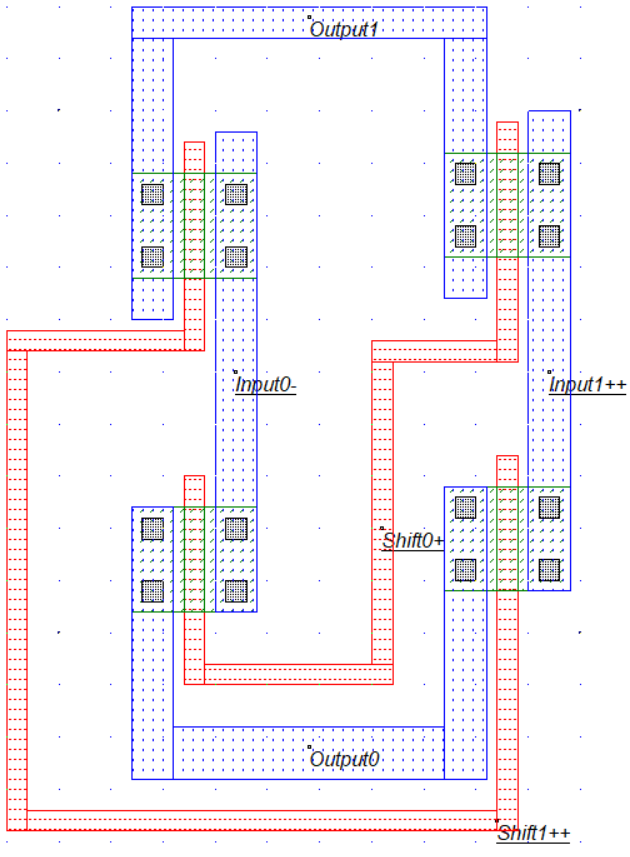
\includegraphics[width=1\linewidth]{Images/2b}
		\caption{2X2 Barrel Shifter}
		\label{fig:2b}
	\end{figure}
	\subsection{2X2 Crossbar Switch}
		\begin{figure}[H]
		\centering
		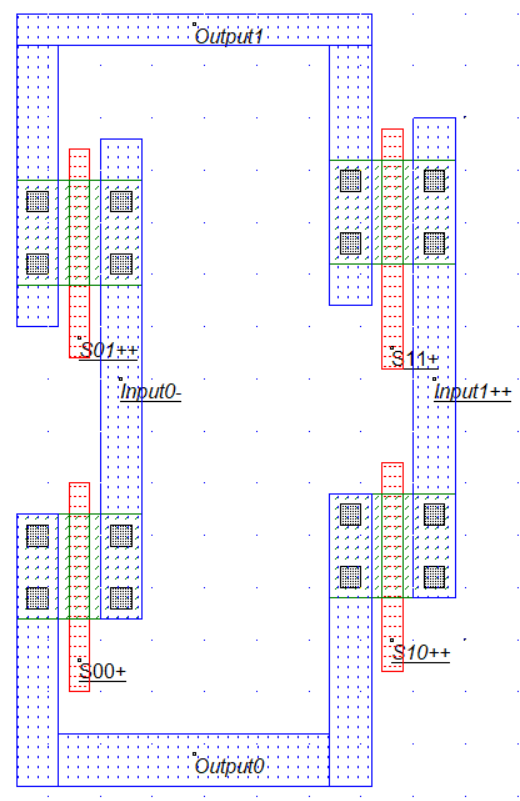
\includegraphics[width=0.9\linewidth]{Images/2c}
		\caption{2X2 Crossbar Switch}
		\label{fig:2b}
	\end{figure}
	\subsection{3X3 Barrel Shifter}
		\begin{figure}[H]
		\centering
		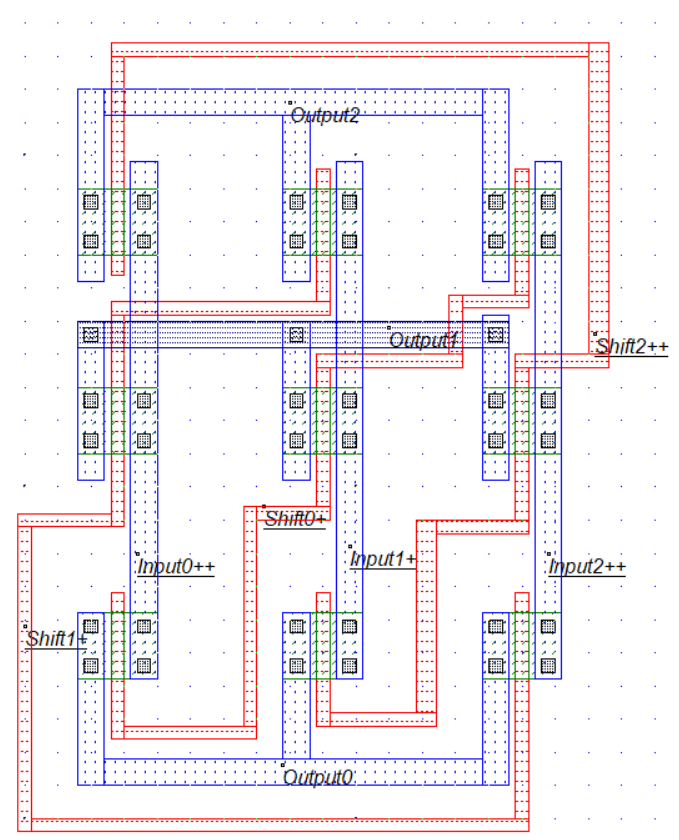
\includegraphics[width=1.1\linewidth]{Images/3B}
		\caption{3X3 Barrel Shifter}
		\label{fig:2b}
	\end{figure}
	\subsection{3x3 Crossbar Switch}
		\begin{figure}[H]
		\centering
		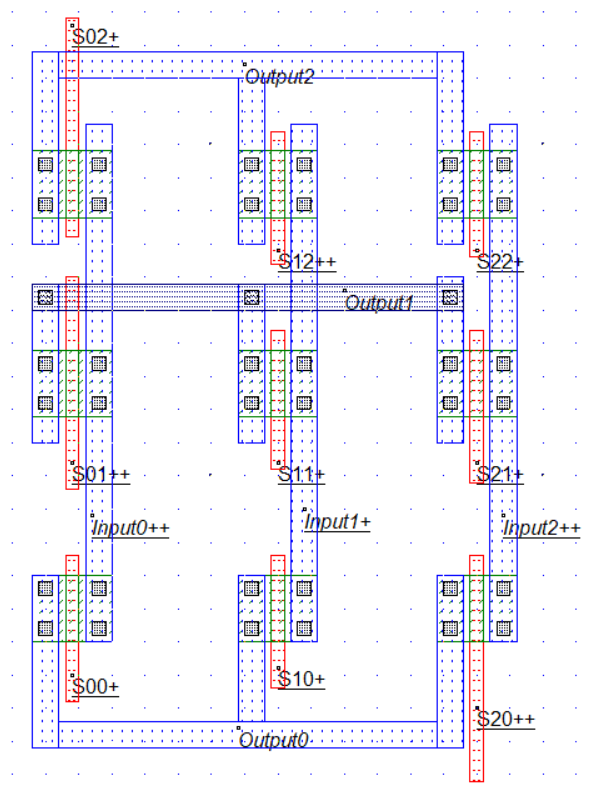
\includegraphics[width=1.1\linewidth]{Images/3c}
		\caption{3X3 Crossbar Switch}
		\label{fig:2b}
	\end{figure}
	\section{Specification}
	
		\begin{table}[H]
		\centering
		\caption{MOSFET Dimensions for nMOS and pMOS Transistors}
		\label{tab:MOSFET_dimensions}
		\begin{tabular}{|c|c|c|c|c|}
			\hline
			\textbf{MOS} & \textbf{\begin{tabular}[c]{@{}c@{}}Width\\ ($\mu m$)\end{tabular}} & \textbf{\begin{tabular}[c]{@{}c@{}}Length\\ ($\mu m$)\end{tabular}} & \textbf{\begin{tabular}[c]{@{}c@{}}Width\\ ($\lambda$)\end{tabular}} & \textbf{\begin{tabular}[c]{@{}c@{}}Length\\ ($\lambda$)\end{tabular}} \\ \hline
			nMOS & 0.600 & 0.120 & 10 & 2 \\ \hline
		\end{tabular}
	\end{table}
		\begin{table}[H]
		\centering
		\caption{Parameters for Vdd+ and Vss- }
		\begin{tabular}{|c|c|c|}
			\hline
			\textbf{Parameter} & \textbf{Value} & \textbf{Unit} \\ \hline
			Vdd+               & 5.00           & $V $            \\ \hline
			Vss-               & 0.00           & $V$             \\ \hline
		\end{tabular}
		
	\end{table}
	% Please add the following required packages to your document preamble:
	% \usepackage{multirow}
	\begin{table}[H]
		\centering
		\caption{Parameters for 2X2 Shifter }
		\begin{tabular}{|c|c|c|c|c|c|}
			\hline
			\textbf{2X2}                                                  & \textbf{\begin{tabular}[c]{@{}c@{}}Input0\\ (V)\end{tabular}} & \textbf{\begin{tabular}[c]{@{}c@{}}Input1\\ (V)\end{tabular}} & \textbf{Shifting} & \textbf{\begin{tabular}[c]{@{}c@{}}Activation Voltage\\  (5.00V)\end{tabular}} & \textbf{\begin{tabular}[c]{@{}c@{}}Activation Voltage\\ (0.00V)\end{tabular}} \\ \hline
			\begin{tabular}[c]{@{}c@{}}2X2 Crossbar Switch\end{tabular} & 0.00                                                          & 5.00                                                          & 1 Bit             & S01,S10                                                                        & S00,S11                                                                       \\ \hline
			\multirow{2}{*}{2X2 Barrel Shifter}                           & 0.00                                                          & 5.00                                                          & 0 Bit             & Shift0                                                                         & Shift1                                                                        \\ \cline{2-6} 
			& 0.00                                                          & 5.00                                                          & 1 Bit             & Shift1                                                                         & Shift0                                                                        \\ \hline
		\end{tabular}
	\end{table}
	
% Please add the following required packages to your document preamble:
% \usepackage{multirow}
\begin{table}[H]
		\centering
	\caption{Parameters for 3X3 Shifter }
	\scalebox{.95}{
\begin{tabular}{|c|c|c|l|c|c|c|}
	\hline
	\textbf{3X3}                                                                   & \textbf{\begin{tabular}[c]{@{}c@{}}Input0\\ (V)\end{tabular}} & \textbf{\begin{tabular}[c]{@{}c@{}}Input1\\ (V)\end{tabular}} & \multicolumn{1}{c|}{\textbf{\begin{tabular}[c]{@{}c@{}}Input2\\ (V)\end{tabular}}} & \textbf{Shifting} & \textbf{\begin{tabular}[c]{@{}c@{}}Activation Voltage\\  (5.00V)\end{tabular}} & \textbf{\begin{tabular}[c]{@{}c@{}}Activation Voltage\\ (0.00V)\end{tabular}} \\ \hline
	\begin{tabular}[c]{@{}c@{}}3X3\\  Crossbar Switch\end{tabular}                 & 5.00                                                          & 0.00                                                          & 5.00                                                                               & 1 Bit             & S01,S12,S20                                                                    & \begin{tabular}[c]{@{}c@{}}S00,S02,S10,\\ S11,S21,S22\end{tabular}            \\ \hline
	\multirow{3}{*}{\begin{tabular}[c]{@{}c@{}}3X3\\  Barrel Shifter\end{tabular}} & 5.00                                                          & 0.00                                                          & 5.00                                                                               & 0 Bit             & Shift0                                                                         & Shift1,Shift2                                                                 \\ \cline{2-7} 
	& 5.00                                                          & 0.00                                                          & 5.00                                                                               & 1 Bit             & Shift1                                                                         & Shift0,Shift2                                                                 \\ \cline{2-7} 
	& \multicolumn{1}{l|}{5.00}                                     & \multicolumn{1}{l|}{0.00}                                     & 5.00                                                                               & 2 Bit             & Shift 2                                                                        & Shift0,Shift1                                                                 \\ \hline
	\end{tabular}}
\end{table}


	\newpage
	\section{Output Waveshape }
	\subsection{2X2 Barrel Shifter}
		\begin{figure}[H]
		\centering
		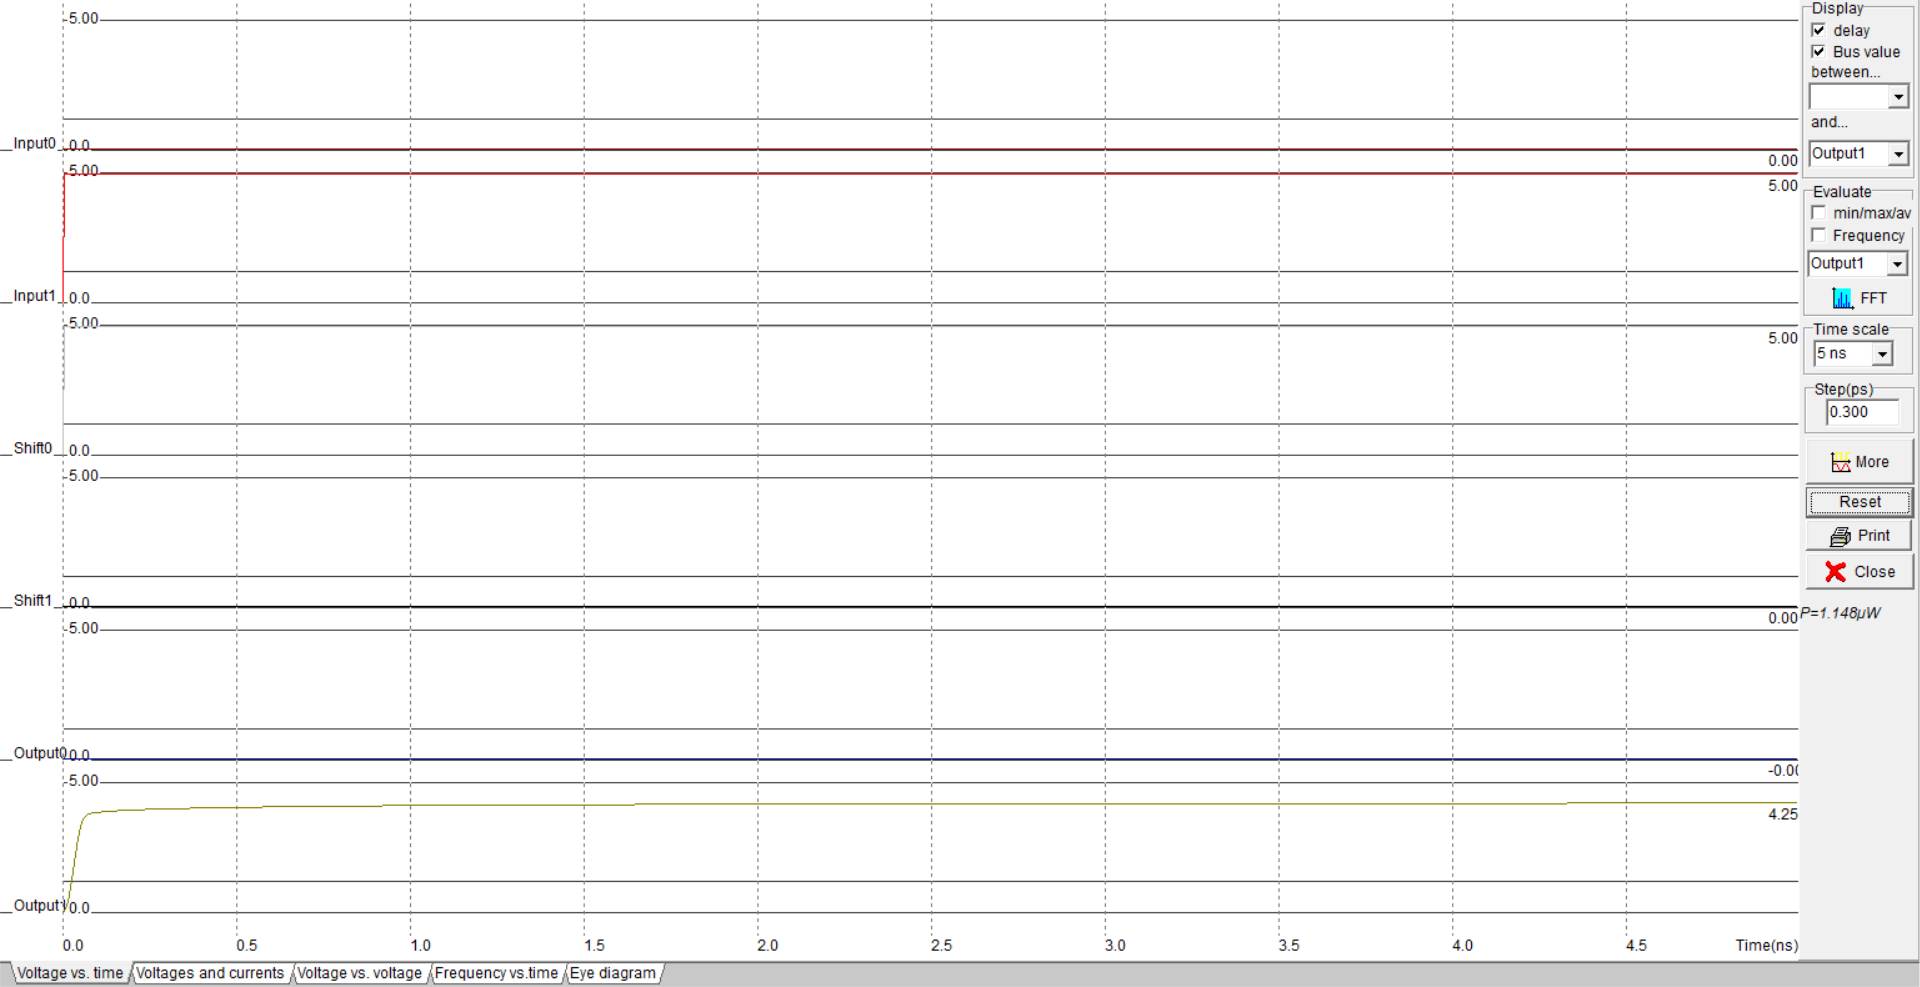
\includegraphics[width=1\linewidth, height=.4\textheight]{Images/2bs0}
		\caption{Output Waveshape 2X2 Barrel Shifter (O Bit Shift)}
		\label{fig:2b}
	\end{figure}
	
		\begin{figure}[H]
		\centering
		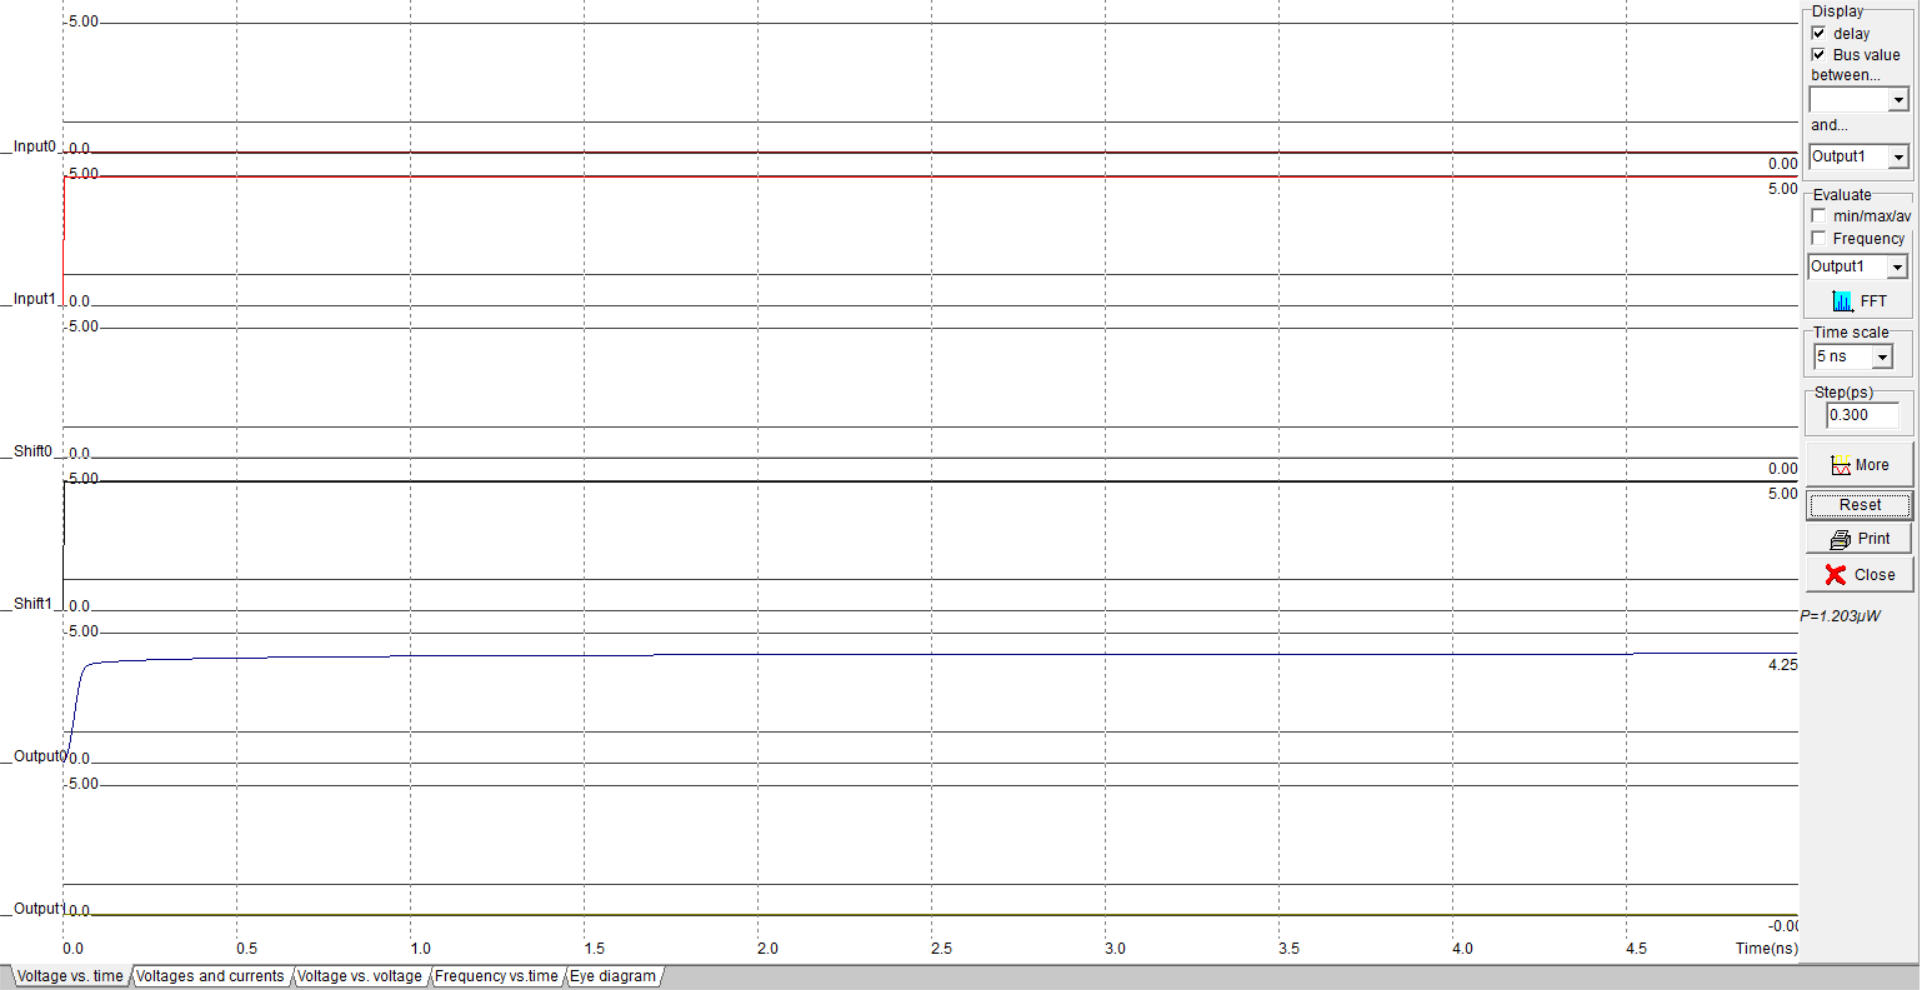
\includegraphics[width=1\linewidth, height=.4\textheight]{Images/2bs1}
		\caption{Output Waveshape 2X2 Barrel Shifter (1 Bit Shift)}
		\label{fig:2b}
	\end{figure}
	
	
	\subsection{2X2 Crossbar Switch}
		\begin{figure}[H]
		\centering
		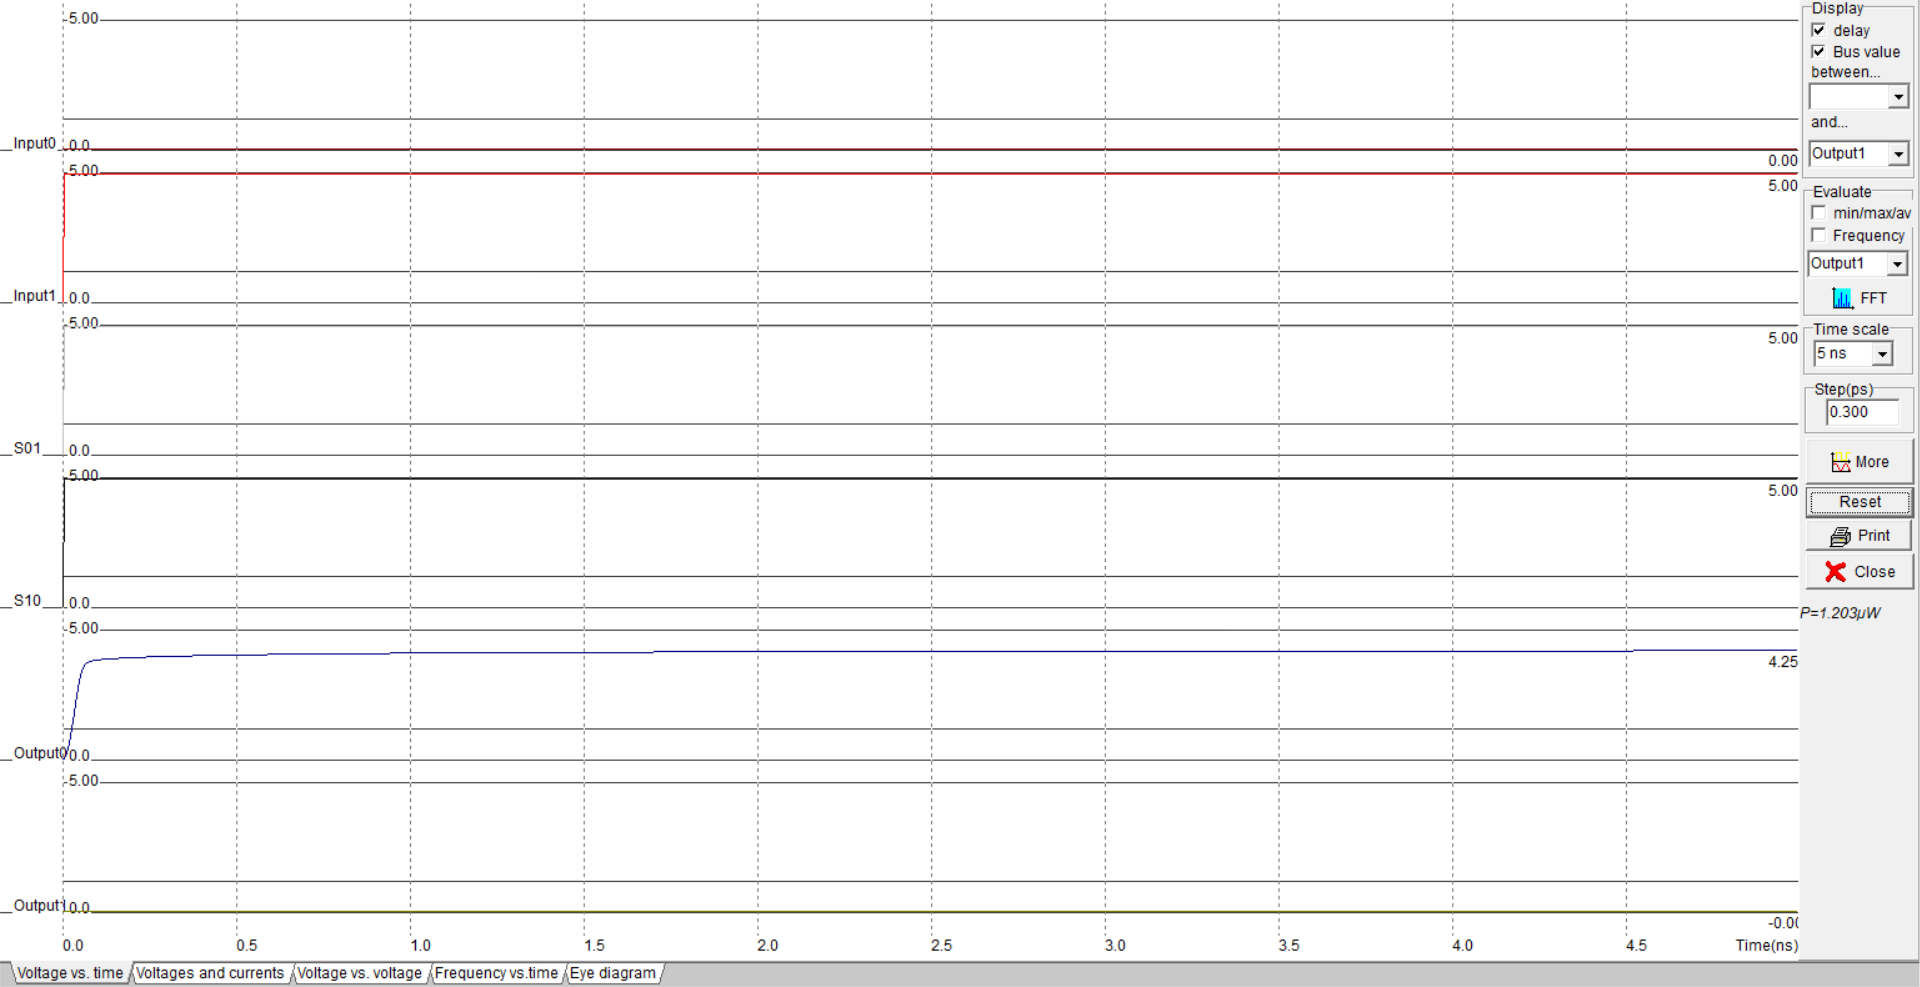
\includegraphics[width=1\linewidth, height=.39\textheight]{Images/2cs1}
		\caption{Output Waveshape 2X2 Crossbar Switch (1 Bit Shift)}
		\label{fig:2b}
	\end{figure}
	\subsection{3x3 Crossbar Switch}
		\begin{figure}[H]
		\centering
		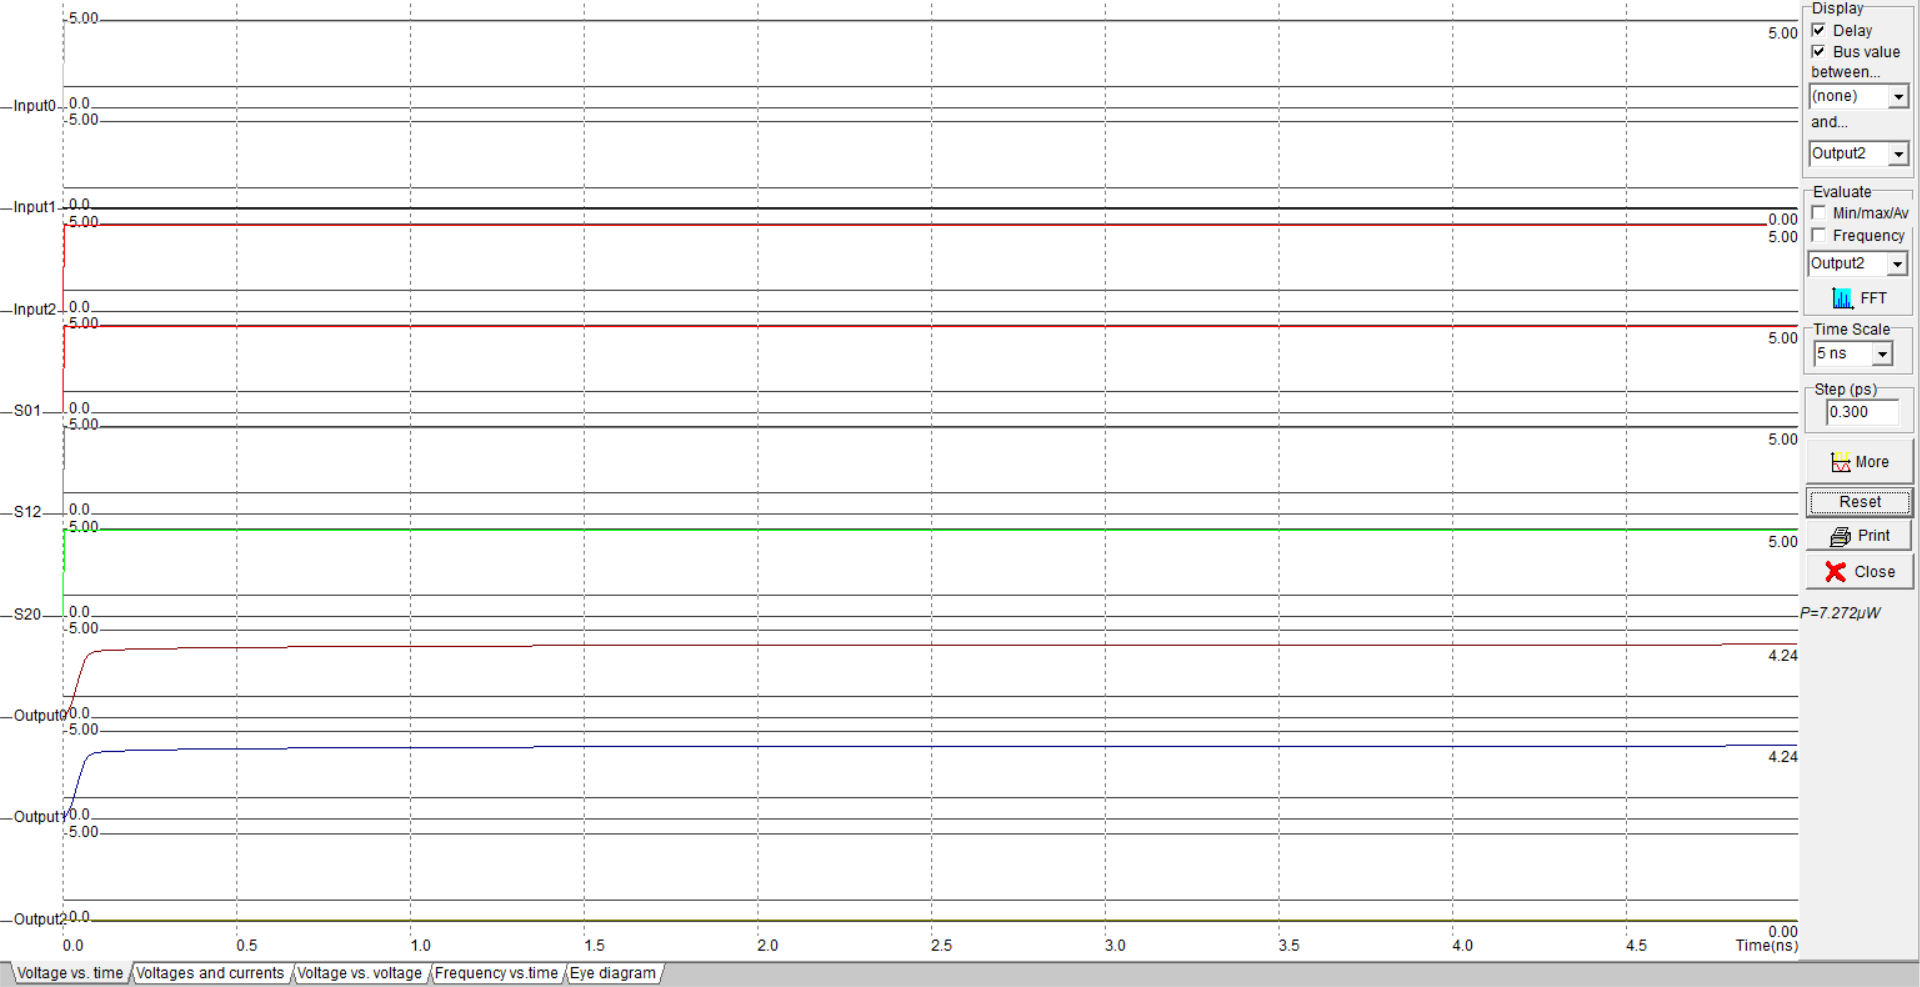
\includegraphics[width=1\linewidth, height=.41\textheight]{Images/3cs2}
		\caption{Output Waveshape 3X3 Crossbar Switch (1 Bit Shift)}
		\label{fig:2b}
	\end{figure}
	\subsection{3X3 Barrel Shifter}
		\begin{figure}[H]
		\centering
		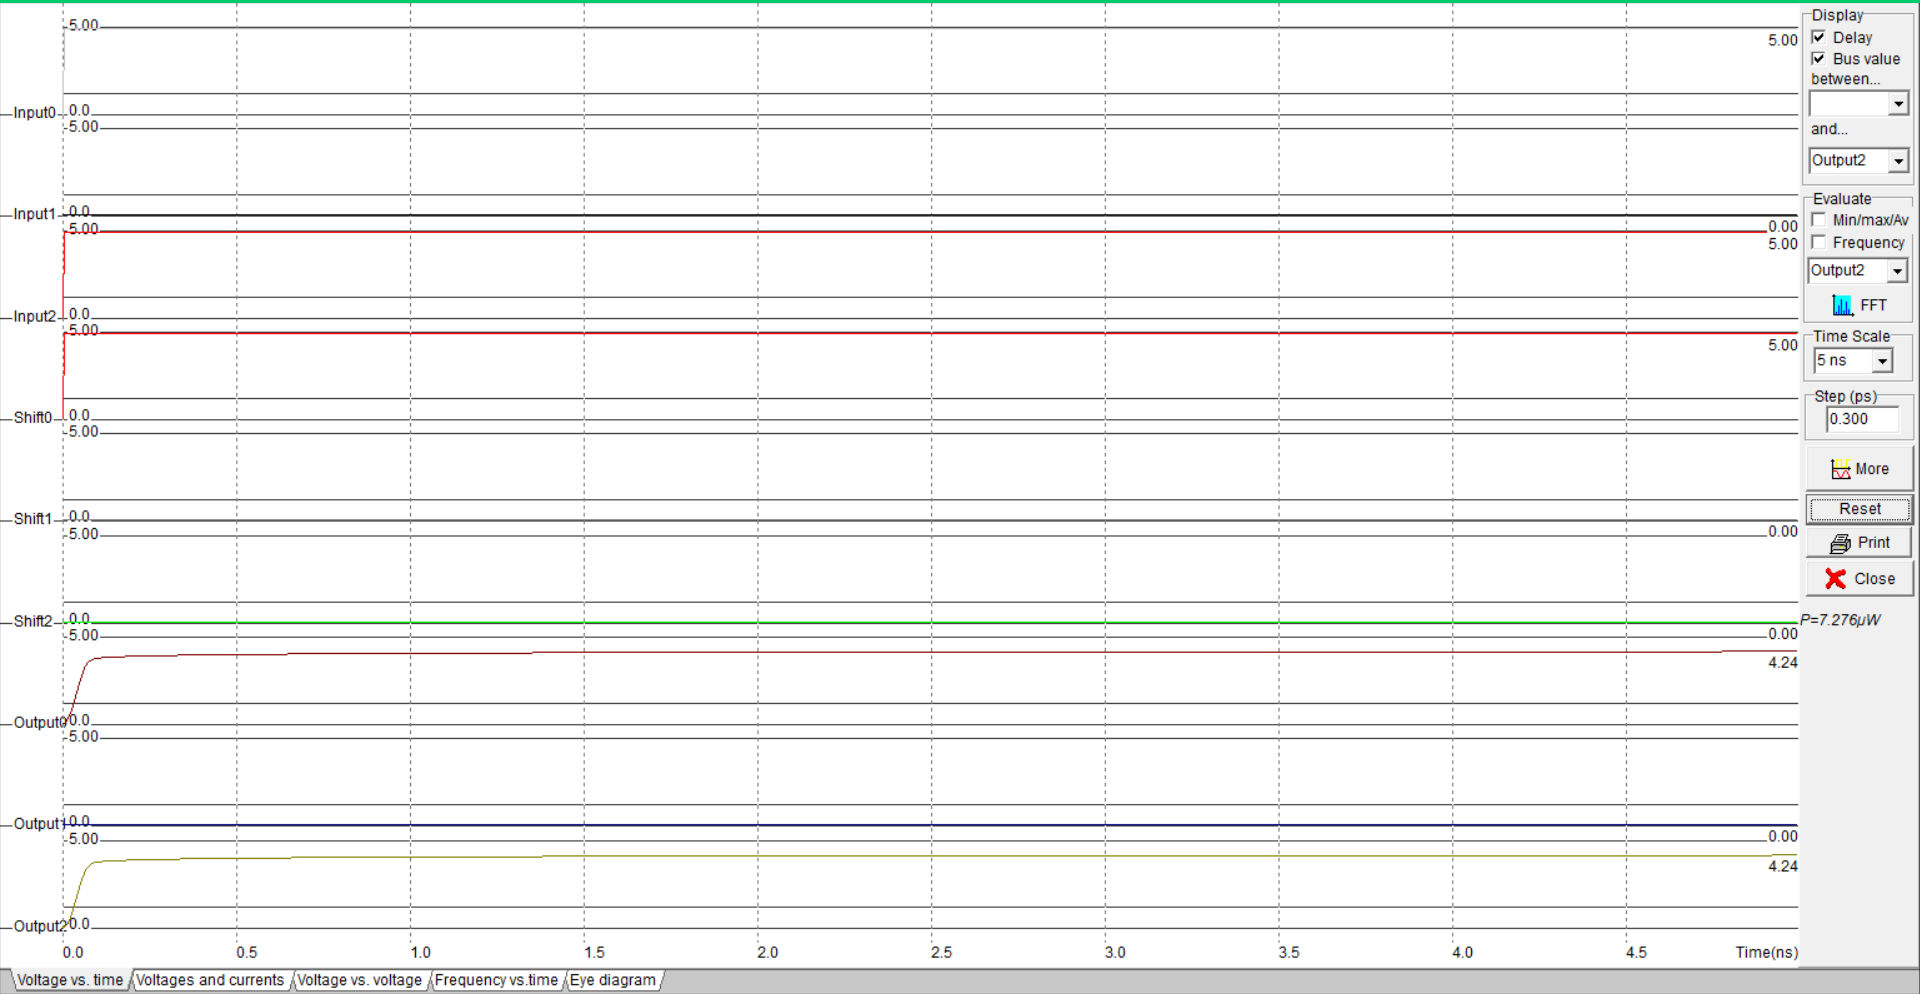
\includegraphics[width=1\linewidth, height=.42\textheight]{Images/3bs0}
		\caption{Output Waveshape 3X3 Barrel Shifter (0 Bit Shift)}
		\label{fig:2b}
	\end{figure}
	
	\begin{figure}[H]
		\centering
		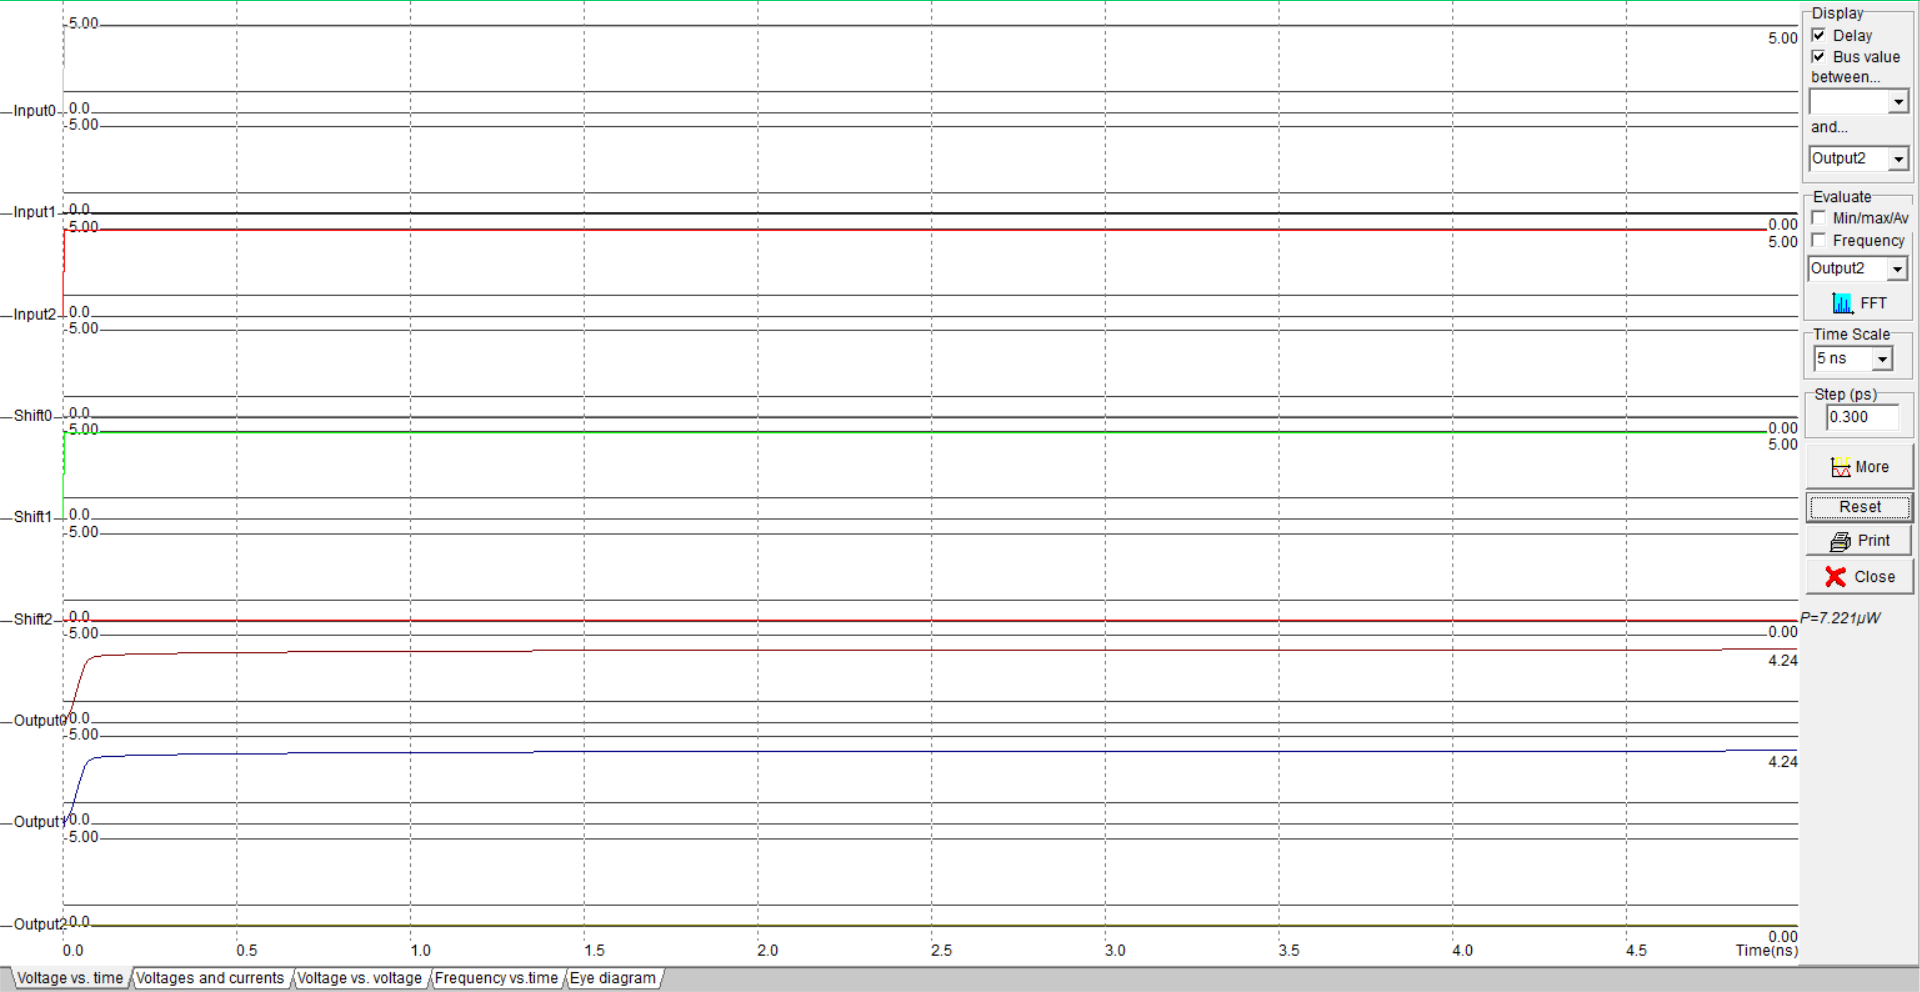
\includegraphics[width=1\linewidth, height=.42\textheight]{Images/3bs1}
		\caption{Output Waveshape 3X3 Barrel Shifter (1 Bit Shift)}
		\label{fig:2b}
	\end{figure}
	
	\begin{figure}[H]
		\centering
		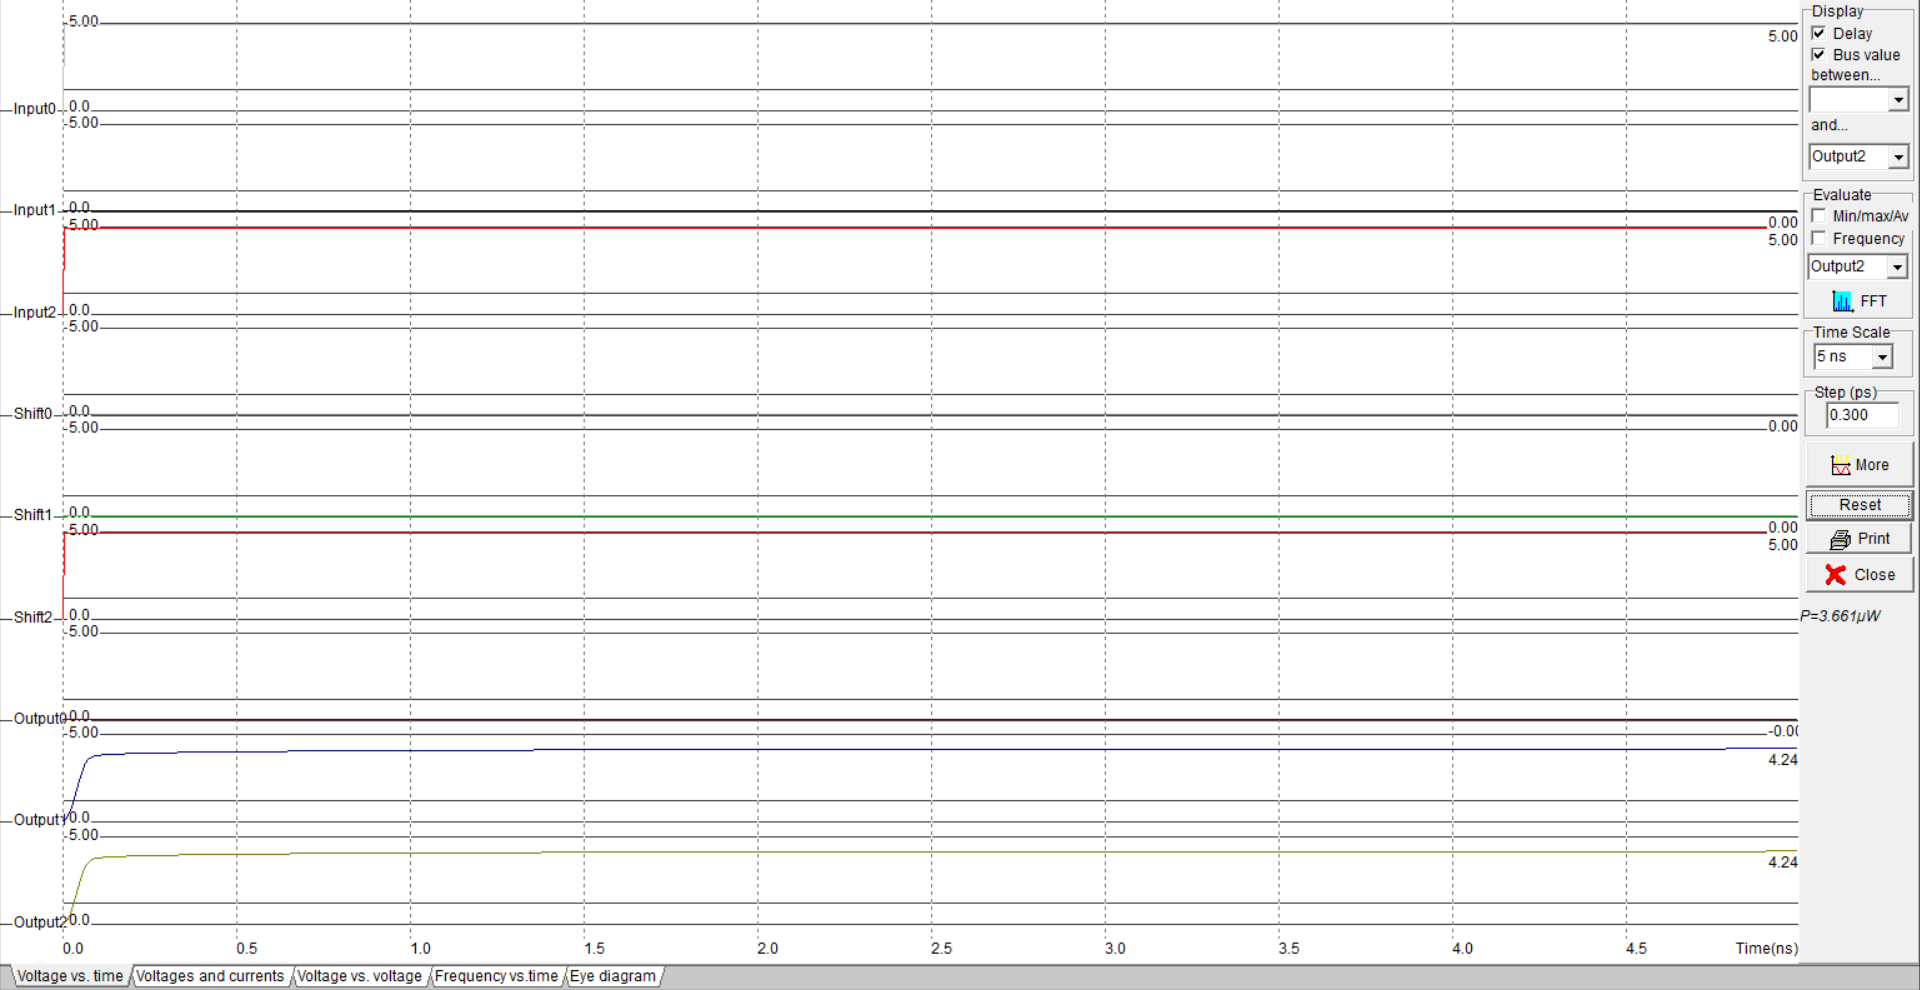
\includegraphics[width=1\linewidth, height=.42\textheight]{Images/3bs2}
		\caption{Output Waveshape 3X3 Barrel Shifter (2 Bit Shift)}
		\label{fig:2b}
	\end{figure}

	\section{Discussion }
	
	In the lab, the barrel shifter and crossbar switch circuits were designed to efficiently shift data to the right by a specified number of positions in a single operation. The implementation of the 2x2 and 3x3 barrel shifters was achieved, allowing data to be shifted by 0, 1, or 2 bits. It was noted that shifting data in the barrel shifter was easier due to having fewer control lines compared to the crossbar switch.
	
	On the other hand, the 2x2 and 3x3 crossbar switches produced outputs similar to those of the barrel shifter, but controlling the shifting lines was more challenging. We had to give High voltage (5V) to each gate of the nMOS transistors according to the desired bit shifting.

	
	
	
\end{document}